% !TeX root = ../main.tex

\chapter{整体设计}
\label{cha:chapter02}
本项目选择把跳跃和滑翔分开作为两个独立的过程来分析与控制,用一个无刷电机驱动跳跃部分,用一个舵机控制机翼的开合。
\section{理论计算}
\label{sec:calculations}
取$g=9.8m/s^2$,预计机器人重量$m=200g$,跳跃高度$h=1m$,起跳电机做功时间$t=0.1s$,则机器人所需最小动能:
\begin{equation}
\label{equ:chap2:W_calc}
W_k=mgh
\end{equation}
二级齿轮减速器机械效率估计为$\eta=80\%$,则所需电机输出最小平均功率:
\begin{equation}
  \label{equ:chap2:P_calc}
  \bar{P}_{min}=\frac{W_k}{t·\eta}
  \end{equation}
解得:$$\bar{P}_{min}=24.5(W)$$
二级齿轮减速器减速比大约在10\sim30:1,设计中一次起跳输出级齿轮大约需要转半圈,取减速比20:1,则所需无刷电机转速:
$$\omega_{min}=0.5\times10\div t\times60=6000(rpm)$$
使用2S锂离子电池,额定电压$V=7.4V$,则所需最小电机KV值:
$$KV_{min}=\omega_{min}\div V=810(rpm/V)$$
一般来讲KV值越小无刷电机转矩越大,根据计算及机械需求考虑,选择了最大功率$P_{max}=168W$的朗宇X2305航模无刷电机,KV值$KV=1450$。\\
机器人起跳最小速度:
\begin{equation}
  \label{equ:chap2:v_calc}
  v=\sqrt{2gh}
  \end{equation}
根据动量定理:
\begin{equation}
  \label{equ:chap2:motion_principle}
  \bar{F}·t=m·v
  \end{equation}
解得所需平均力:$$\bar{F}=8.854(N)$$
航模用无刷电机的力矩数据不好获得,我们通过相同工作条件下的带螺旋桨升力进行估算,实际输出力只会更大。电机参数显示6000rpm时的升力等效质量约为$m_f=200\sim300g$,即经减速器输出的力为:$$F_min=m_{f,min}·g·20=39.2(N)>\bar{F}$$
此处还未考虑腿部连杆结构带来的机械增益,而其均值应>1,因此理论上输出力是足够支持跳跃的。
\section{元件选型}
\label{sec:components}
根据上述计算过程与现实考量,选择元件如表\ref{tab:bom}所示。
\begin{table}[htb]
  \centering
  \begin{minipage}[t]{0.8\linewidth}
  \caption{BOM表}
  \label{tab:bom}
    \begin{tabularx}{\linewidth}{lX}
      \toprule[1.5pt]
      {\heiti 元件名} & {\heiti 描述} \\\midrule[1pt]
      朗宇X2305无刷电机 & 外转子无刷电机,KV值1450 \\
      NanoPi Duo2 开发板 & 全志H3主控,运行Ubuntu 18.04\\
      FOC电机控制板 &  基于STSPINF0A方案的BLDC矢量控制 \\
      EMAX 2S航模锂电池 & 容量300mAh,质量为15g\\
      DS-S002M 4.3g数字舵机 & 用于控制机翼开合\\
      OV5640摄像头 & 500W像素,1080p@30fps,720p@60fps\\
      \bottomrule[1.5pt]
    \end{tabularx}
  \end{minipage}
\end{table}

\begin{figure}[H]
  \centering
  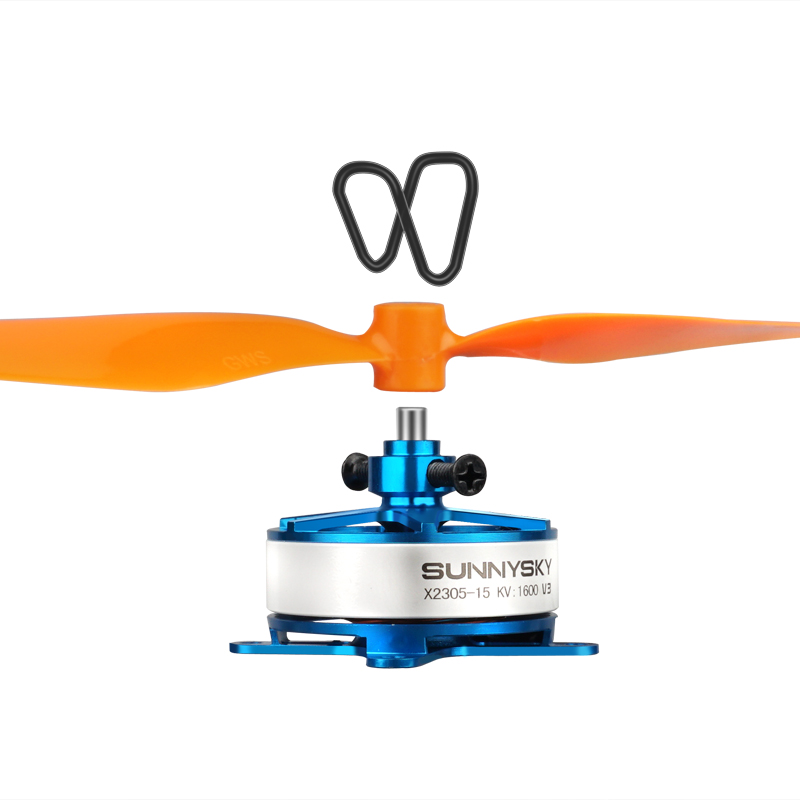
\includegraphics[height=10cm]{X2305.png}
  \caption{朗宇X2305无刷电机}
  \label{fig:X2305}
\end{figure}
\begin{figure}[H]
  \centering
  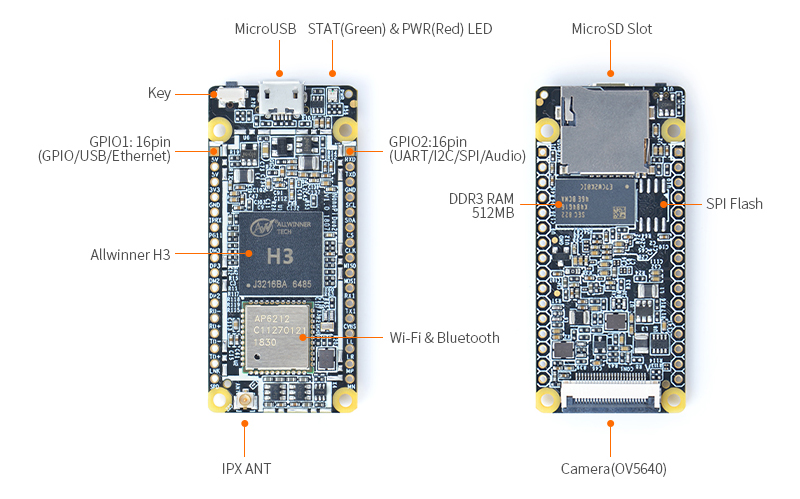
\includegraphics[height=10cm]{NanoPi-Duo2.jpg}
  \caption{NanoPi Duo2 开发板}
  \label{fig:Pi}
\end{figure}
\begin{figure}[H]
  \centering
  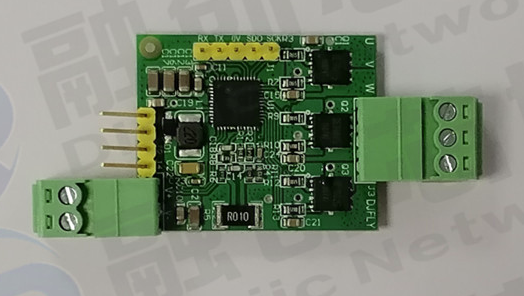
\includegraphics[height=7cm]{FOC.png}
  \caption{FOC电机控制板}
  \label{fig:FOC_board}
\end{figure}
\begin{figure}[H]
  \centering
  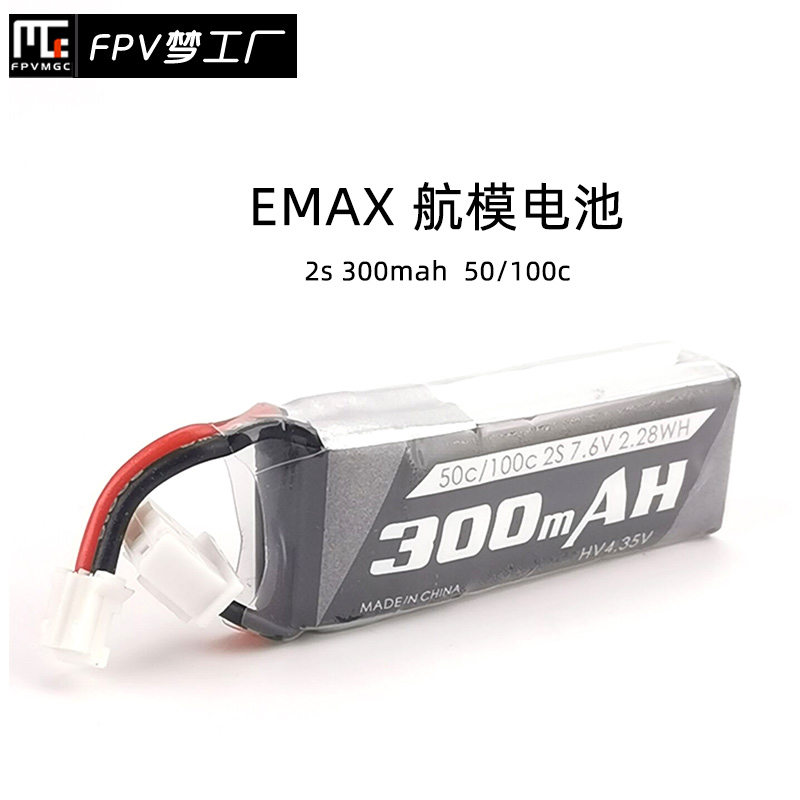
\includegraphics[height=10cm]{emax.jpg}
  \caption{EMAX 2S航模锂电池}
  \label{fig:emax}
\end{figure}
\begin{figure}[H]
  \centering
  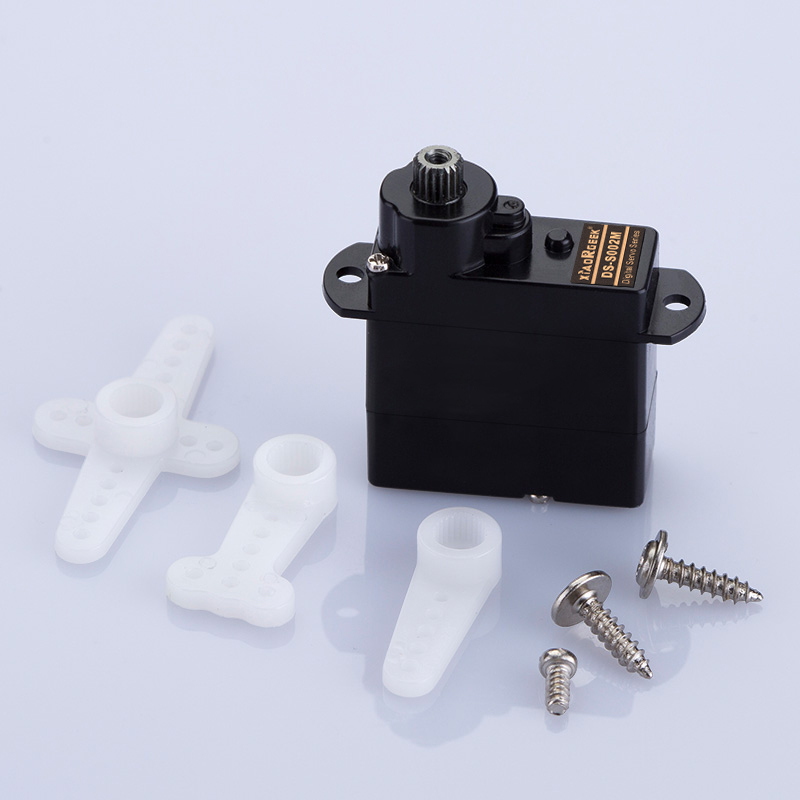
\includegraphics[height=10cm]{servo.jpg}
  \caption{DS-S002M 4.3g数字舵机}
  \label{fig:servo}
\end{figure}
\begin{figure}[H]
  \centering
  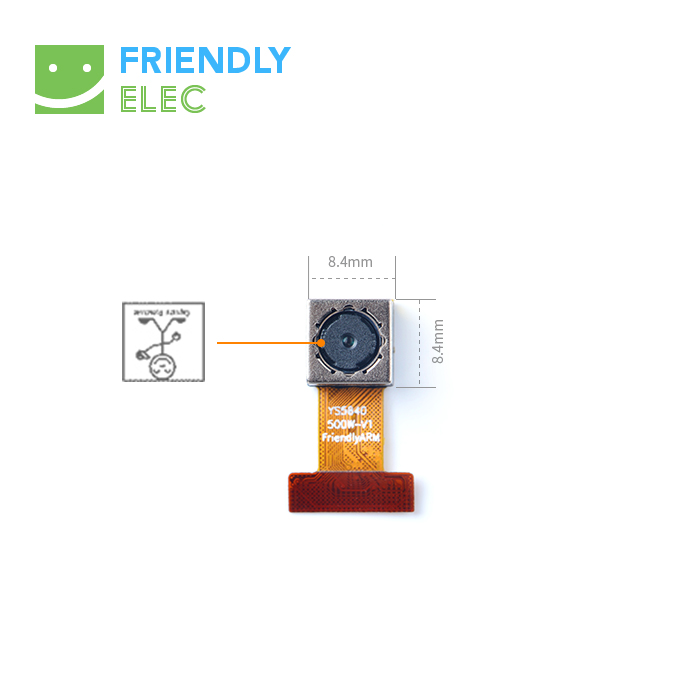
\includegraphics[height=10cm]{OV5640.jpg}
  \caption{OV5640摄像头}
  \label{fig:OV5640}
\end{figure}
\section{机械设计}
\label{sec:mechanical}
初步设计的机器人整体结构三维仿真图如下(螺丝等固定细节略去):
\begin{figure}[H]
  \centering
  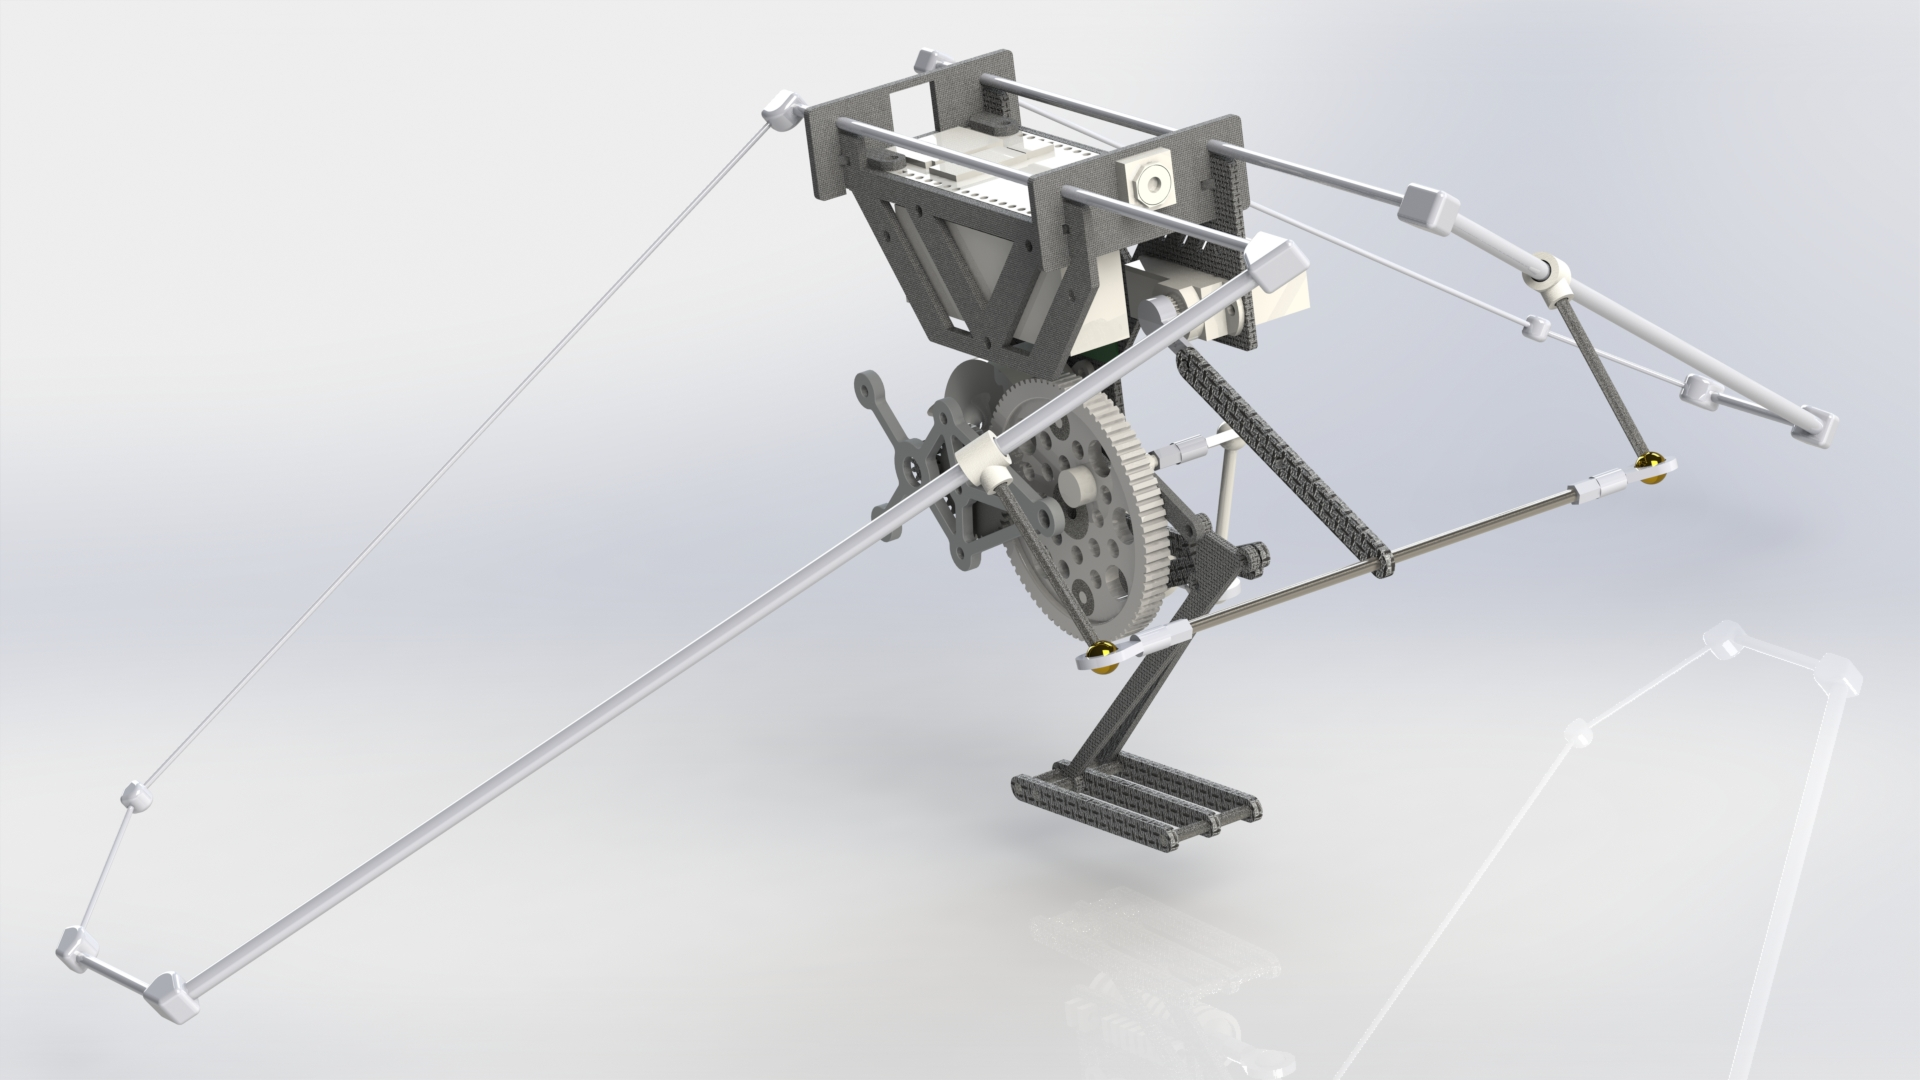
\includegraphics[height=8cm]{render2.jpg}
  \caption{整体结构渲染图}
  \label{fig:render_v1}
\end{figure}
\subsection{减速器设计}
设计目标为减速比20:1的两级齿轮减速器。考虑本项目实际尺寸,选用模数为0.5或0.6的齿轮较为合适。在市面上可直接买到的齿轮中,选择了0.5模数15齿的主轴齿轮,10/36齿的次级双层齿轮和80齿的末级齿轮。其中主轴齿轮材料为铜(粉末铸造),次级齿轮为铁基齿轮,而体积最大的末级齿轮采用了铝合金材质,兼顾了硬度与重量。

\begin{figure}[H]
  \centering
  \subcaptionbox{主轴齿轮\label{fig:cog1}}[4cm] 
    {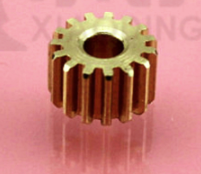
\includegraphics[height=3cm]{cog15.png}}
  \hspace{3em}
  \subcaptionbox{次级齿轮\label{fig:cog2}}[3cm]
      {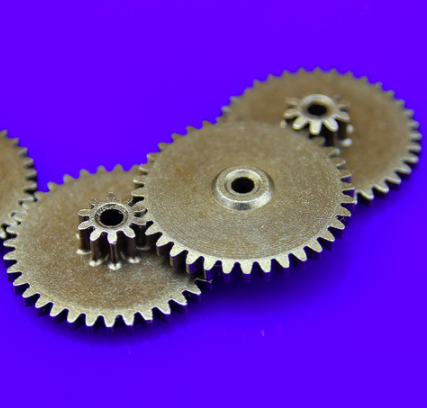
\includegraphics[height=3cm]{cog10_36.png}}
  \hspace{4em}
  \subcaptionbox{末级齿轮\label{fig:cog3}}
      {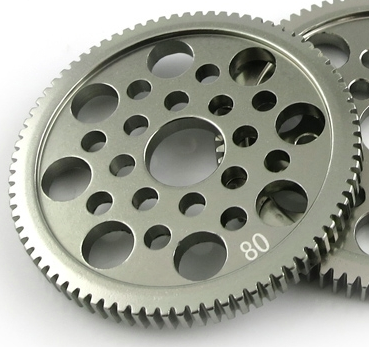
\includegraphics[height=3cm]{cog80.png}}
  \caption{齿轮的选择}
  \label{fig:cogs}

\end{figure}
实际减速比为:$$i=36\div15\times80\div10=19.2$$
据此我们设计出用于固定的减速器支架,选择铝合金材质CNC而成,保证连接强度的同时尽量减轻质量。设计图与实物图如图\ref{fig:retarder}所示,装配示意图如图\ref{fig:retarder_assembly}所示。
\begin{figure}[H]
  \centering
  \subcaptionbox{减速器模型\label{fig:retarder_model}}[7cm] 
    {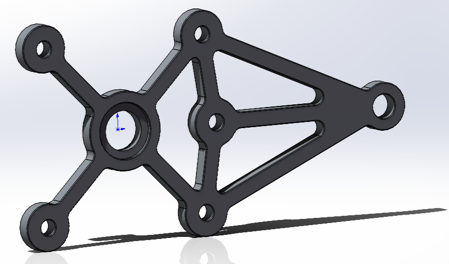
\includegraphics[height=4cm]{retarder_model.png}}
  \hspace{4em}
  \subcaptionbox{减速器实物\label{fig:retarder_real}}
      {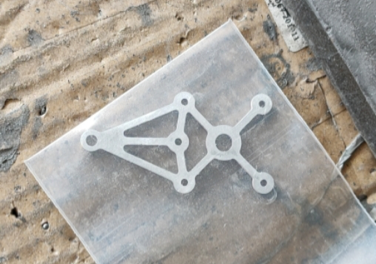
\includegraphics[height=4cm]{retarder_real.png}}
  \caption{减速器}
  \label{fig:retarder}
\end{figure}
\begin{figure}[H]
  \centering%
  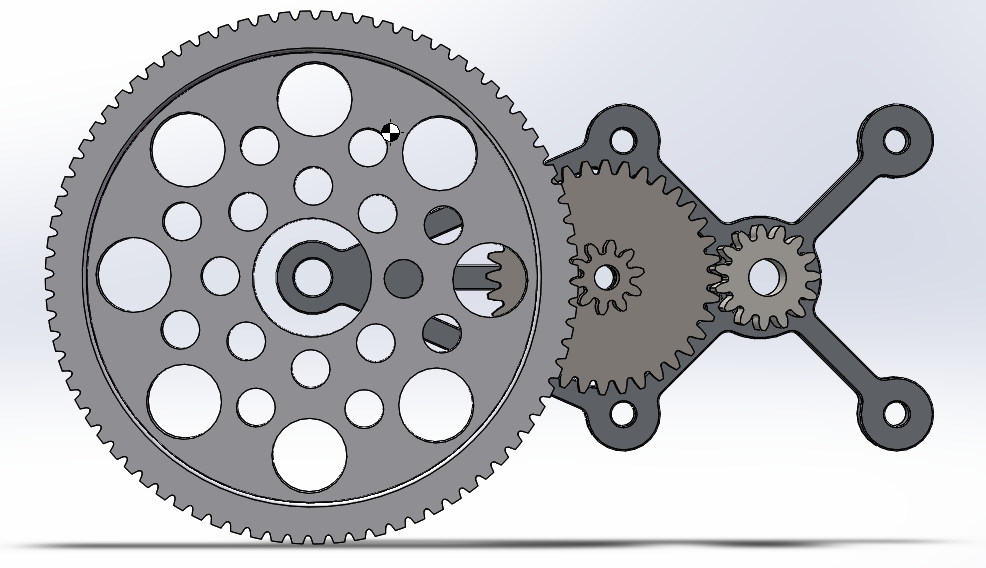
\includegraphics[height=8cm]{retarder_assembly.png}
  \caption{减速器装配图}
  \label{fig:retarder_assembly}
\end{figure}
\subsection{腿部设计}
参考Salto\cite{Salto}的腿部模型,此处实现了如图\ref{fig:2d_leg_fold}和图\ref{fig:2d_leg_stretch}所示的连杆结构。其中灰色圆为输出级齿轮,带动上部的曲柄-摇臂四连杆结构,同时四连杆摇臂为一凹四边形块,与机身相连的另一点在下部又组成了一个平行四边形四连杆,在输出级利用杠杆结构增大位移,实现触地端的较大速度,从而使身体跳起。虽然看上去略显复杂,但总体形态接近自然界大多数生物的腿部构造,这也从一个侧面反映了该结构的合理性。

\begin{figure}[H]
  \centering%
  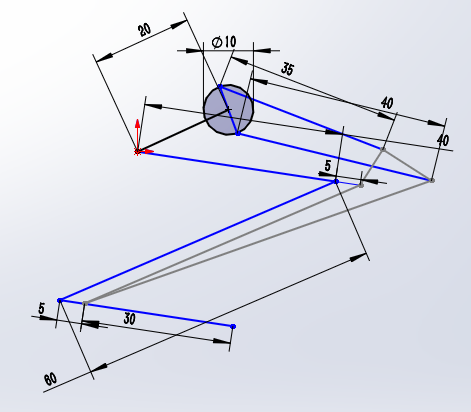
\includegraphics[height=6cm]{2d_leg_fold.png}
  \caption{起跳前准备姿势}
  \label{fig:2d_leg_fold}
\end{figure}
\begin{figure}[H]
  \centering%
  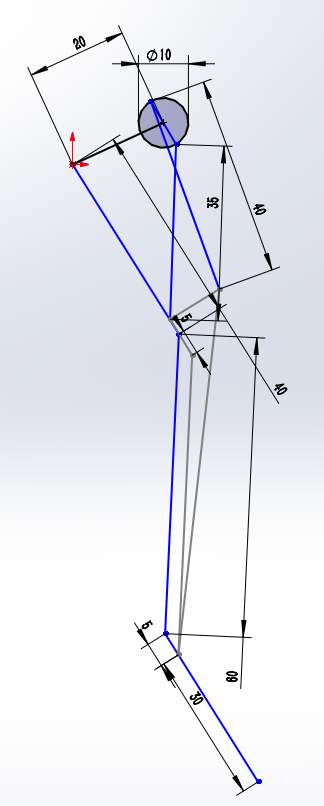
\includegraphics[height=11cm]{2d_leg_stretch.png}
  \caption{起跳后空中姿势}
  \label{fig:2d_leg_stretch}
\end{figure}

据此尺寸在SolidWorks中设计出三维模型,装配示意图如图\ref{fig:3d_leg}所示。
\begin{figure}[H]
  \centering%
  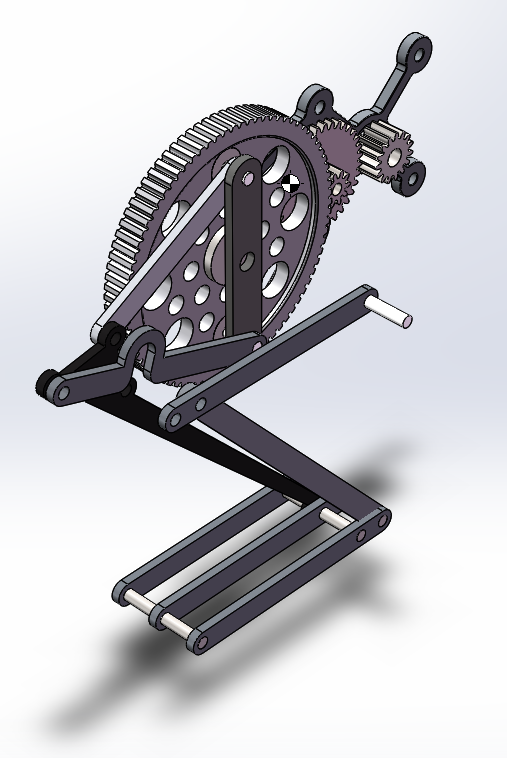
\includegraphics[height=8cm]{3d_leg.png}
  \caption{腿部装配图}
  \label{fig:3d_leg}
\end{figure}

\subsection{机翼设计}
\label{sec:wings}
采用蝴蝶式\cite{EPFL}折叠机翼设计,利用一个小舵机带动两片机翼的同步开合。为了降低机翼质量,采用碳纤维骨架与蒙皮的形式,骨架由碳纤维杆与3D打印的接头组成,翼面材料使用潍坊风筝布料,以保证强度与抗老化性。机翼部分设计模型如图\ref{fig:wings_mechanism}所示。
\begin{figure}[H]
  \centering%
  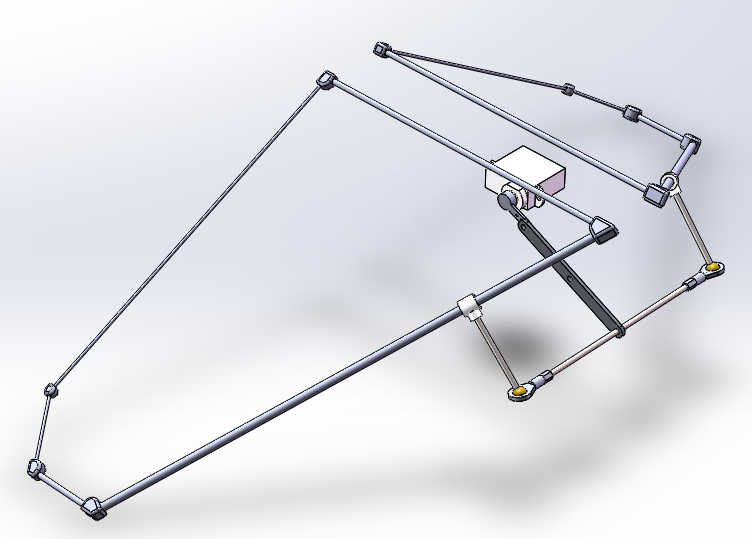
\includegraphics[height=8cm]{wings_mechanism.png}
  \caption{机翼原理图}
  \label{fig:wings_mechanism}
\end{figure}

\subsection{机身设计}
机身设计目标:实现腿、机翼和其他元件的可靠连接。
\begin{figure}[H]
  \centering%
  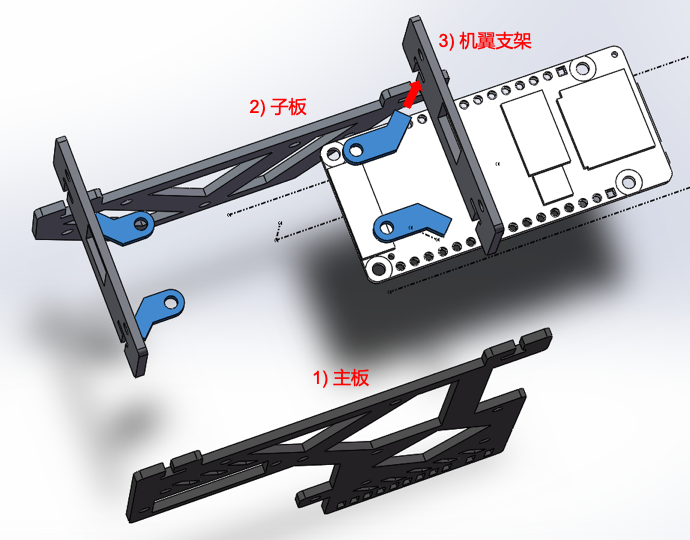
\includegraphics[height=10cm]{mt_exploded_marked.png}
  \caption{榫卯结构爆炸视图}
  \label{fig:mt_exploded}
\end{figure}
为了降低制造难度,我们希望所有的设计都尽可能是平面的。而在三维世界中实现二维平面物体之间的连接,就要使用一些连接结构。为了降低装配难度及提高鲁棒性(在如此小的体积上拧螺丝也并非易事),在机身主板与各子板之间的连接设计上参考了我国古代人民智慧的结晶——榫卯结构。如图\ref{fig:mt_exploded}所示,蓝色楔子即为榫头,2号子板与3号机翼支架之间的空隙构成了榫眼,红色箭头标出了楔子的运动方向。装配好的结构如图\ref{fig:mt_assembled}所示。此时四角的楔子与主控板以螺丝螺母紧固,使得三个方向的平面得以可靠连接,同时并未使用除电路板四个螺丝孔以外的任何螺丝安装,实现了简洁而高效的机械结构。
\begin{figure}[H]
  \centering
  {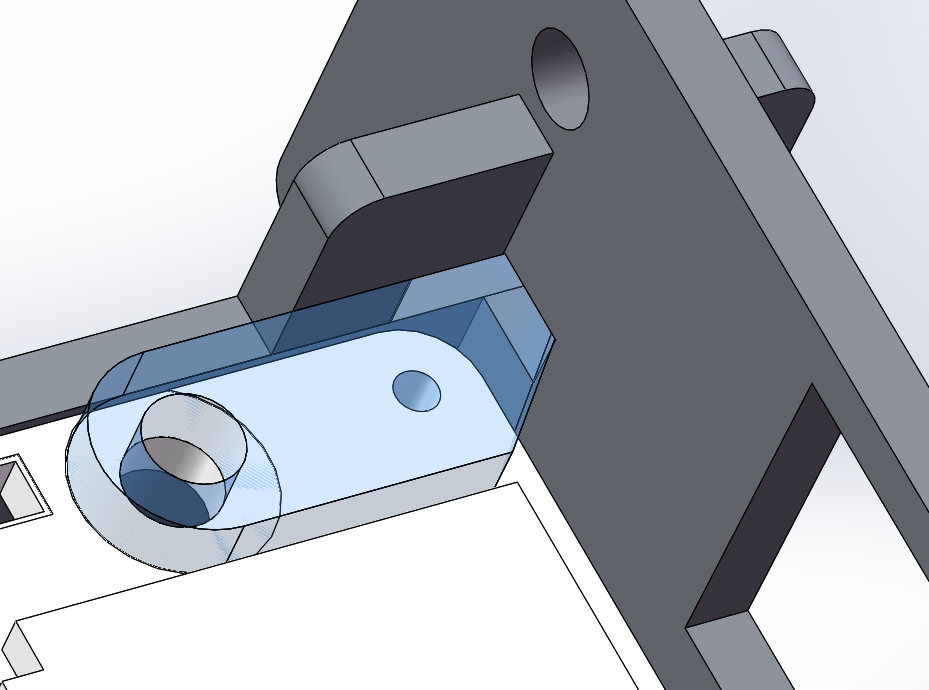
\includegraphics[height=10cm]{mt_zoom.png}}
  \caption{榫卯连接处透视图}
  \label{fig:mt_zoom}
\end{figure}
\begin{figure}[H]
  \centering
  {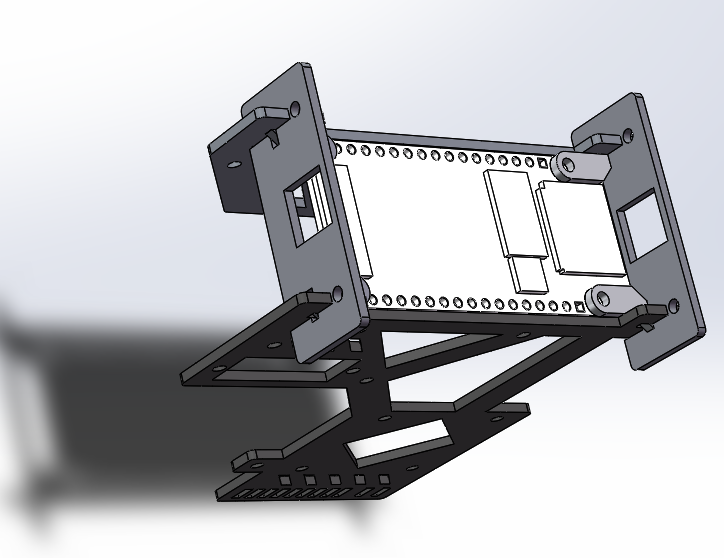
\includegraphics[height=10cm]{mt_assembled.png}}
  \caption{主板、子板、机翼支架和电路板装配完成}
  \label{fig:mt_assembled}
\end{figure}
\subsection{磁助力装置}
为了增加起跳时的爆发力,设计了如图\ref{fig:magnet_fold}、\ref{fig:magnet_jump}所示的磁助力装置。机器人下蹲时电机需要克服磁力做功,相当于将能量存储到磁场中。
\begin{figure}[H]
  \centering
  {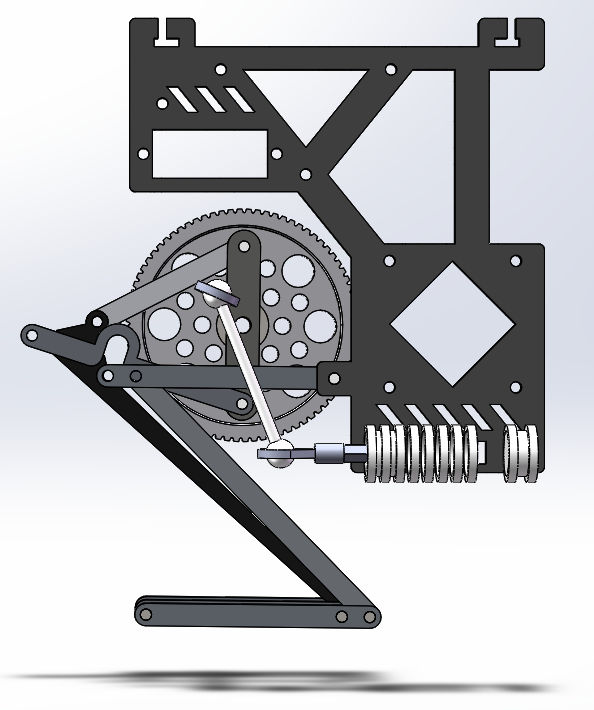
\includegraphics[height=7cm]{magnet_fold.png}}
  \caption{折叠状态磁场储能}
  \label{fig:magnet_fold}
\end{figure}
\begin{figure}[H]
  \centering
  {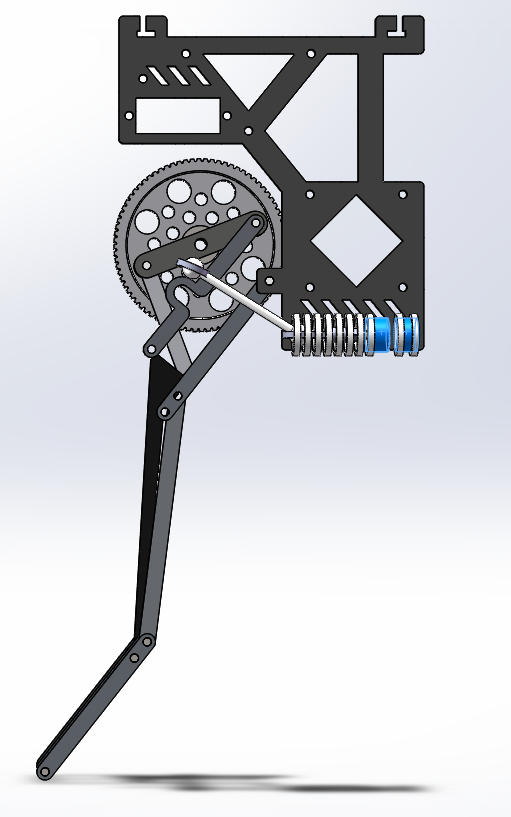
\includegraphics[height=10cm]{magnet_jump.png}}
  \caption{跳跃时磁场做功}
  \label{fig:magnet_jump}
\end{figure}
\subsection{整体装配图}
机身全部装配图如下:
\begin{figure}[H]
  \centering
  {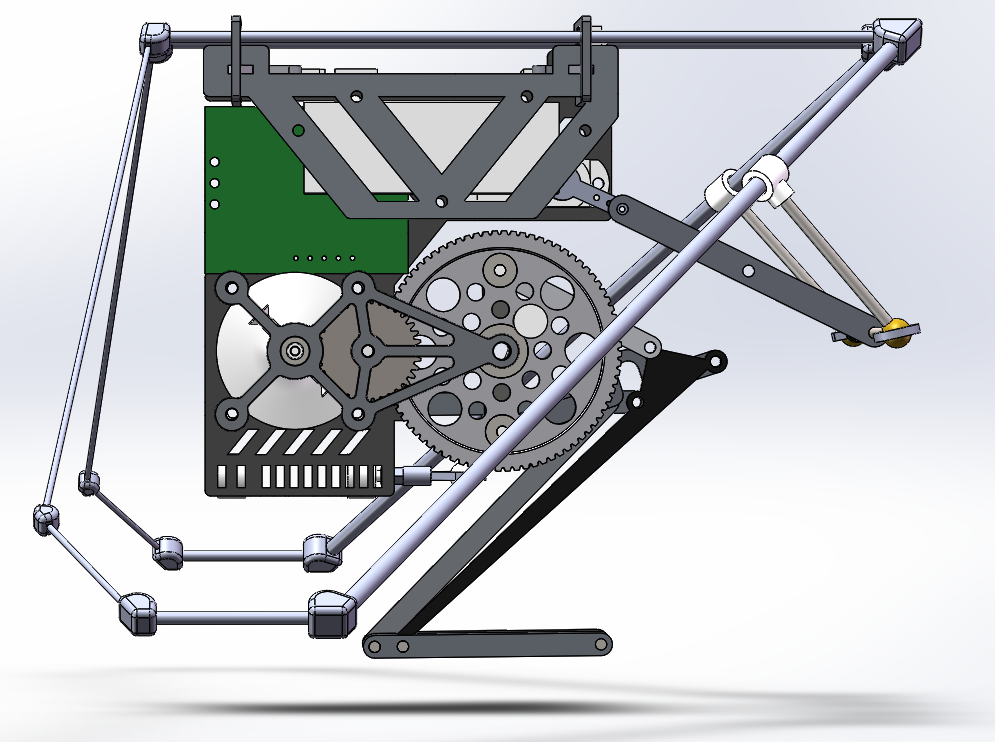
\includegraphics[height=10cm]{left.png}}
  \caption{左视图}
  \label{fig:left}
\end{figure}
\begin{figure}[H]
  \centering
  {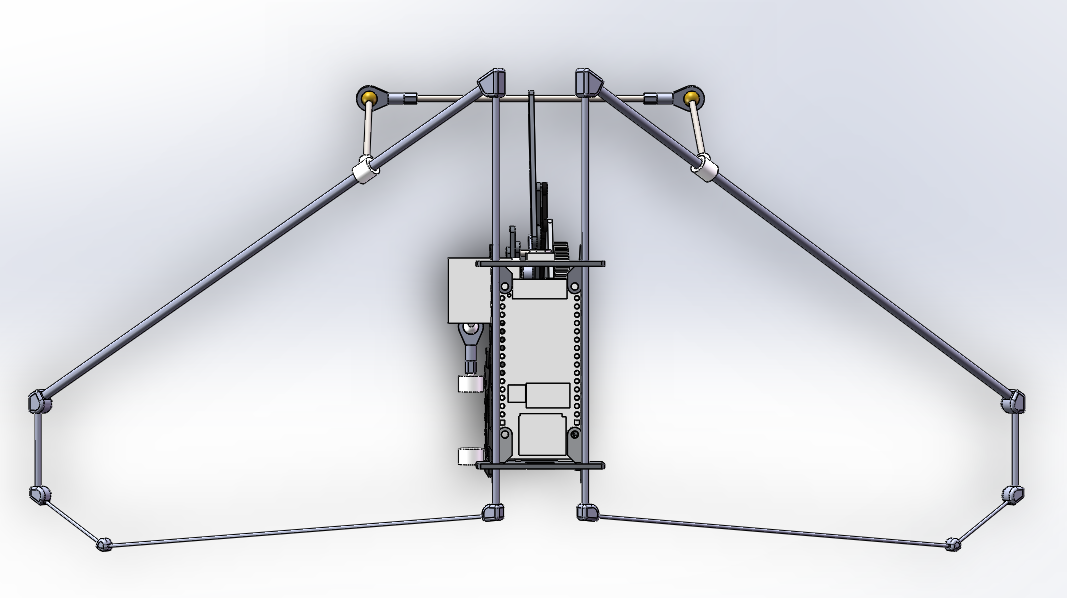
\includegraphics[height=8cm]{up.png}}
  \caption{俯视图}
  \label{fig:up}
\end{figure}
\begin{figure}[H]
  \centering
  {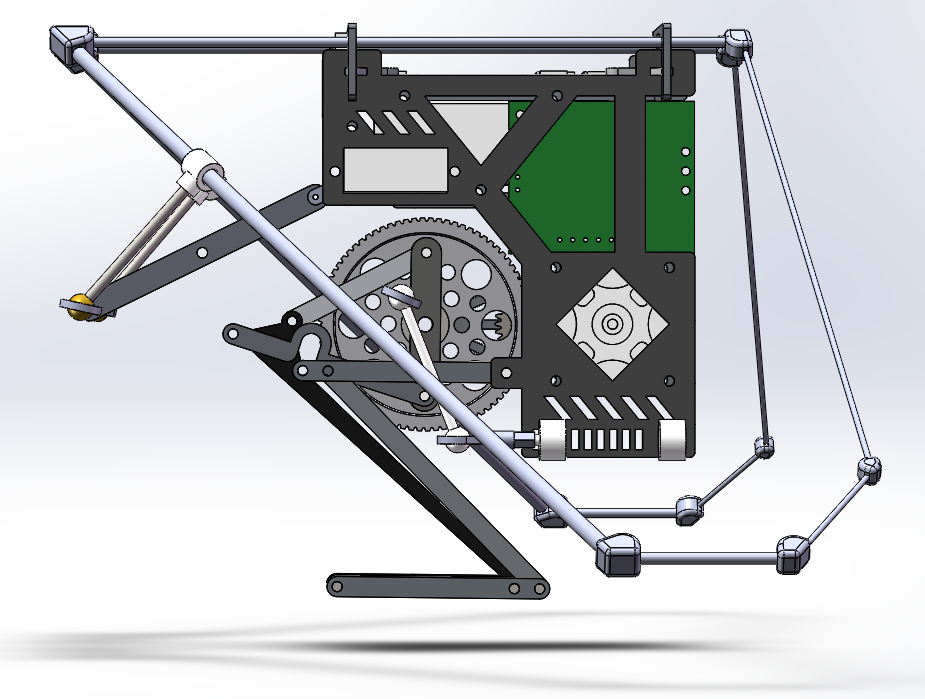
\includegraphics[height=11cm]{right.png}}
  \caption{右视图}
  \label{fig:right}
\end{figure}
\begin{figure}[H]
  \centering
  {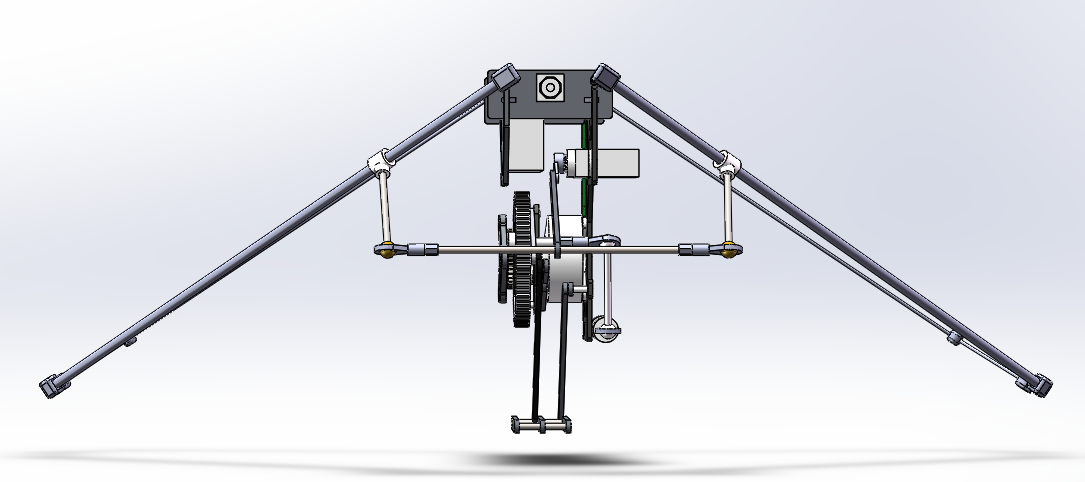
\includegraphics[height=7cm]{front.png}}
  \caption{正视图}
  \label{fig:front}
\end{figure}
\begin{figure}[H]
  \centering
  {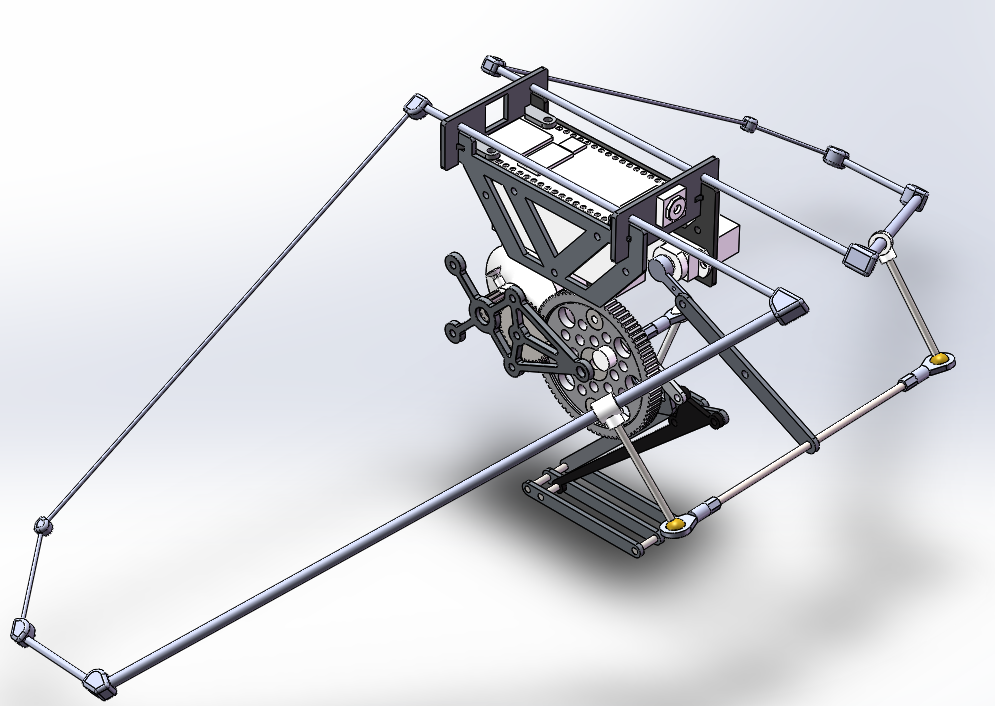
\includegraphics[height=10cm]{leftup.png}}
  \caption{左上等轴测视图}
  \label{fig:leftup}
\end{figure}
\begin{figure}[H]
  \centering
  {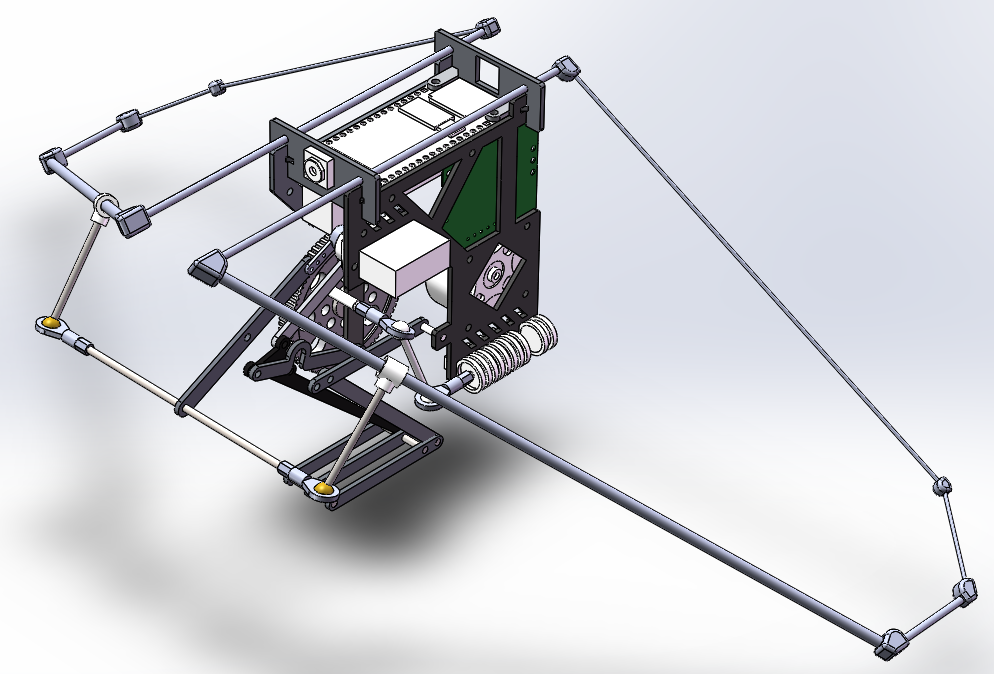
\includegraphics[height=10cm]{rightup.png}}
  \caption{右上等轴测视图}
  \label{fig:rightup}
\end{figure}
\section{嵌入式系统}
电路部分系统架构如图\ref{fig:system_architecture}所示。电源部分,2S锂电池直接接入FOC控制板,FOC控制板上自带稳压芯片提供STSPIN32F0A芯片所需的3.3V;而同时并联一个5V稳压模块,给主控板NanoPi供电。主控板通过UART与FOC控制板通讯,进而控制电机。同时主控板还直接通过PWM控制舵机位置,并通过MIPI接口连接OV5640摄像头,通过Wi-Fi传回实时图像数据。上位机也通过Wi-Fi向机器人发送指令。
\begin{figure}[H]
  \centering
  {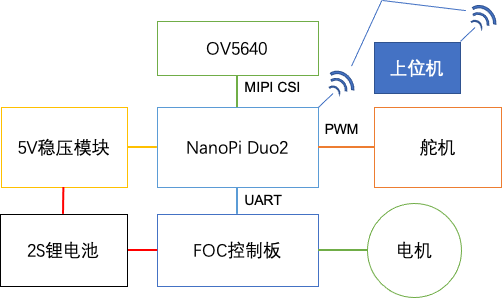
\includegraphics[height=5cm]{system_architecture.png}}
  \caption{系统架构}
  \label{fig:system_architecture}
\end{figure}
\subsection{控制算法}
电机控制部分主要使用了工业上成熟的FOC矢量控制技术\cite{FOC}。FOC的核心思想是使定子电流的磁场始终与转子的磁场正交,从而始终保持扭矩最大。因此其数学基础就是三相坐标系与直角坐标系之间的坐标变换,以及控制理论中的PID控制。而实际情况远比这个简单的理想模型要复杂,因此本项目选择站在前人的肩膀上,使用来自意法半导体的成熟的ST FOC电机库\cite{MCSDK},实现对电机的精确控制。
\begin{figure}[H]
  \centering
  {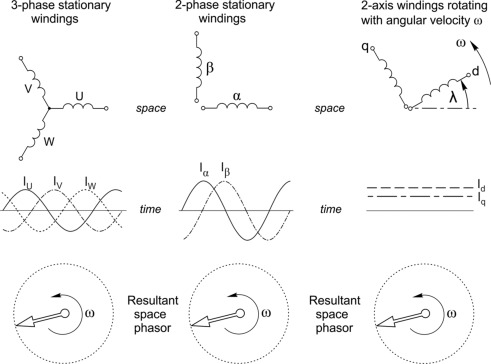
\includegraphics[height=8cm]{FOC.jpg}}
  \caption{FOC电流坐标变换\cite{FOC}}
  \label{fig:FOC}
\end{figure}
如图\ref{fig:FOC}所示,以$\alpha$,$\beta$所在轴建立直角坐标系,投影可得:
$$
  \left\{
  \begin{aligned}
  I_\alpha & = &I_U-cos(\frac{\pi}{3})I_V-cos(\frac{\pi}{3})I_W \\
  I_\beta  & = &sin(\frac{\pi}{3})I_V-sin(\frac{\pi}{3})I_W
  \end{aligned}
  \right.
$$
即:
\begin{equation}
  \label{equ:chap2:clark}
  \left[ \begin{array}{c}
  I_\alpha \\
  I_\beta
  \end{array}
  \right]=K\left[ 
    \begin{array}{ccc}
    1 & -\frac{1}{2} & -\frac{1}{2}\\
    0 & \frac{\sqrt{3}}{2} & -\frac{\sqrt{3}}{2}   
    \end{array}
    \right]\left[ \begin{array}{c}
      I_U \\
      I_V \\
      I_W
      \end{array}
      \right]
\end{equation}
式\ref{equ:chap2:clark}被称为Clark变换。自然地,有:
\begin{equation}
  \label{equ:chap2:clark_inv}
  \left[ \begin{array}{c}
    I_U \\
    I_V \\
    I_W
    \end{array}
    \right]=K\prime\left[ 
    \begin{array}{cc}
    1 & 0 \\
    -\frac{1}{2} & \frac{\sqrt{3}}{2} \\
    -\frac{1}{2} & -\frac{\sqrt{3}}{2}   
    \end{array}
    \right]\left[ \begin{array}{c}
      I_\alpha \\
      I_\beta
      \end{array}
      \right]
\end{equation}
式\ref{equ:chap2:clark_inv}被称为Clark逆变换。Clark正逆变换完成了交流三相坐标系与直角坐标系之间电流的转换,是磁场定向控制的基础。而在图\ref{fig:FOC}的第二部分到第三部分,要完成从静止坐标系到旋转坐标系的变换。由几何关系有:
$$
  \left\{
  \begin{aligned}
  I_d & = & I_\alpha cos(\lambda)+I_\beta sin(\lambda) \\
  I_q & = & -I_\alpha sin(\lambda)+I_\beta cos(\lambda)
  \end{aligned}
  \right.
$$
即:
\begin{equation}
  \label{equ:chap2:park}
  \left[ \begin{array}{c}
  I_d \\
  I_q
  \end{array}
  \right]=\left[ 
    \begin{array}{cc}
    cos(\lambda) & sin(\lambda)\\
    -sin(\lambda) & cos(\lambda)   
    \end{array}
    \right]\left[ \begin{array}{c}
      I_\alpha \\
      I_\beta
      \end{array}
      \right]
\end{equation}
式\ref{equ:chap2:park}被称为Park变换。易得其逆变换公式:
\begin{equation}
  \label{equ:chap2:park_inv}
  \left[ \begin{array}{c}
  I_\alpha \\
  I_\beta
  \end{array}
  \right]=\left[ 
    \begin{array}{cc}
    cos(\lambda) & -sin(\lambda)\\
    sin(\lambda) & cos(\lambda)   
    \end{array}
    \right]\left[ \begin{array}{c}
      I_d \\
      I_q
      \end{array}
      \right]
\end{equation}
而在嵌入式系统上,更注重算法执行的效率,因此三角函数运算多由查表获得。
\subsection{串口通信协议}
ST MotorControl SDK\cite{MCSDK}提供了如图\ref{fig:MCSDK_UI}所示的功能强大的UI,但却并未提供通信协议细节。好在这是一个开源项目,通过阅读SDK源代码,得到串口通信协议如下:
\begin{figure}[h]
  \centering
  {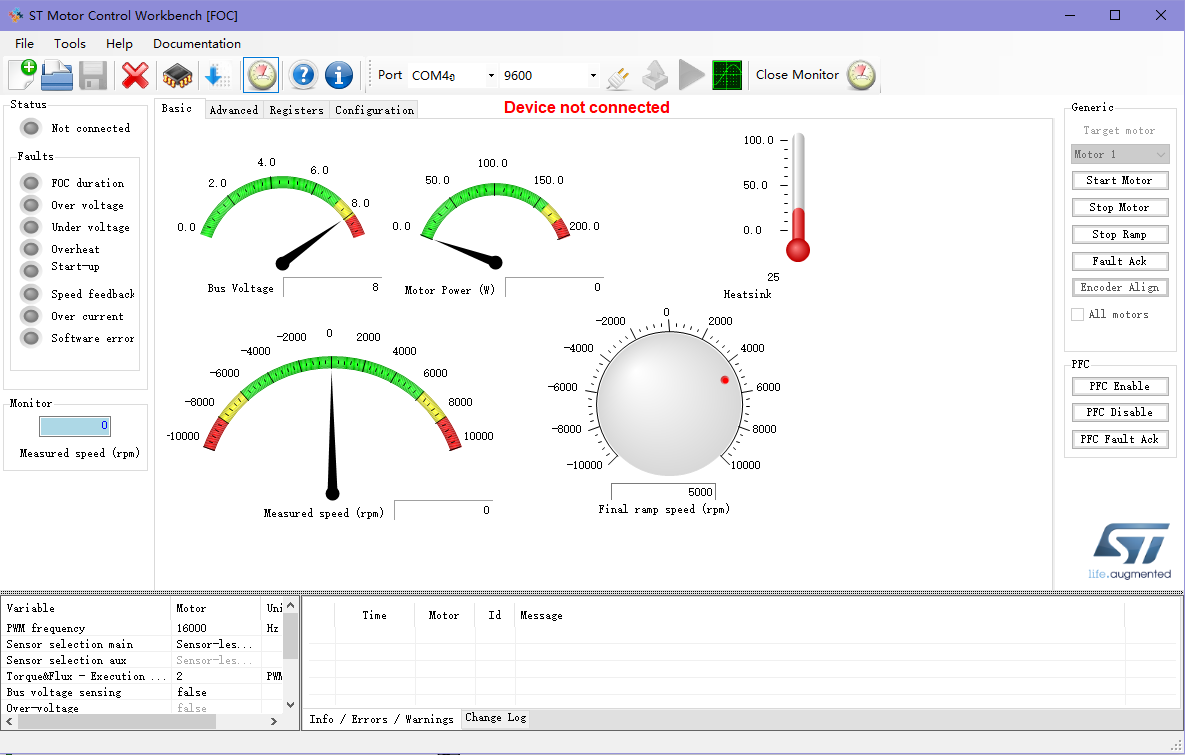
\includegraphics[height=10cm]{MCSDK_UI.png}}
  \caption{MotorControl Workbench上位机\cite{MCSDK}}
  \label{fig:MCSDK_UI}
\end{figure}
\begin{table}[htb]
  \centering
  \begin{minipage}[t]{0.8\linewidth}
  \caption{通信协议(默认波特率9600bps)}
  \label{tab:UART_protocol}
    \begin{tabularx}{\linewidth}{llX}
      \toprule[1.5pt]
      {\heiti 代号} & {\heiti 长度(字节)} & {\heiti 描述} \\\midrule[1pt]
      Code & 1 & 操作码,标识当前数据包的功能 \\
      Size & 1 & 传输负载长度 \\
      Payload & Size & 负载,用于传输命令参数 \\
      CRC & 1 & 校验位\\
      \bottomrule[1.5pt]
    \end{tabularx}
  \end{minipage}
\end{table}
其中校验位的计算方式为将数据包中CRC之前的所有位求和,用一个无符号16位整型变量存储,再把得到的结果的高8位右移8位与低8位相加,得到的结果存入一个8位无符号整型变量(也就是说在最后这步加法中无视溢出)。平心而论,这个操作只能说是魔改的求和校验,并不属于CRC,因为真正的CRC是有纠错能力的,而这个魔改的求和校验码只具有检错能力,因此这个变量名取Parity更为妥当,此处保留了源代码中的变量名。但在这种简单的串口通信中也无须纠错,误码重传代价不大,可以接受。
\subsection{通信系统}
本项目的主要通信框架为ROS\cite{ROS}(Robot Operating System,机器人操作系统)。与Ubuntu 18.04系统对应的ROS版本是ROS Melodic。ROS是一套发布-订阅机制的通信框架,需要一台主机运行roscore作为服务器,其他主机连接到这台服务器来发布和订阅消息。在本项目中主要通过ROS回传摄像头图像数据,可以很方便的在ROS中配置摄像头参数。
\begin{figure}[H]
  \centering
  {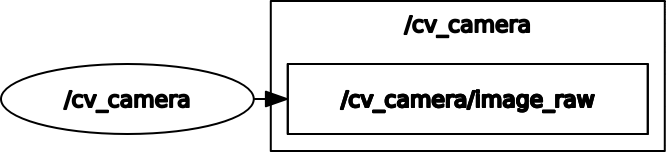
\includegraphics[height=3cm]{rosgraph.png}}
  \caption{ROS节点消息图}
  \label{fig:rosgraph}
\end{figure}